% Foliensatz: "AFu-Kurs nach DJ4UF" von DK0TU, Amateurfunkgruppe der TU Berlin
% Lizenz: CC BY-NC-SA 3.0 de (http://creativecommons.org/licenses/by-nc-sa/3.0/de/)
% Autoren: Sebastian Lange <dl7bst@dk0tu.de>, Lars Weiler <dc4lw@darc.de>

\documentclass[aspectratio=169]{beamer}

\usepackage[ngerman]{babel} % deutsche Worttrennung etc.
\usepackage[utf8]{inputenc} % UTF8 Text

\usepackage[super, comma, numbers, square, sort]{natbib}

\usepackage{hyperref}       % Hyperref Package für bessere Referenzen (todo)
\hypersetup{
	colorlinks=false,       %   false: boxed links; true: colored links
    %linkcolor=white,       %   color of internal links (change box color with linkbordercolor)
    citecolor=red,          %   color of links to bibliography
    filecolor=white,        %   color of file links
    urlcolor=blue           %   color of external links
}

\usepackage{multirow}
\usepackage{wasysym}  % Math Symbols like \permil
%\usepackage{colortbl}
%\usepackage{subscript}
%\usepackage{caption}
%\usepackage{setspace}
%\usepackage{xcolor}        % benutze CodeListe

% Footnote
%\usepackage{hanging}
%
%\setbeamertemplate{footnote}{%
%  \hangpara{2em}{1}%
%  \makebox[2em][l]{\insertfootnotemark}\footnotesize\insertfootnotetext\par%
%}


%\usepackage{pgf}
%\usepackage{tikz}
%\usetikzlibrary{arrows,automata}
%\usetikzlibrary{positioning}
%
%\tikzset{
%    state/.style={
%           rectangle,
%           rounded corners,
%           draw=black, very thick,
%           minimum height=2em,
%           minimum width=2pt,
%           inner sep=2pt,
%           text centered,
%           },
%}

%\usepackage{listings}
%\lstset{basicstyle=\small, numberstyle=\tiny, extendedchars=true, numbers=left, numbersep=5pt}
%\lstset{showtabs=false, showspaces=false, showstringspaces=false}
%%\lstset{backgroundcolor=\color{white!75!lightgray}, , frame=single}
%%\lstset{backgroundcolor=\color{white}}
%%\lstset{backgroundcolor=none}
%\lstset{keywordstyle=\color{blue!50!gray},  identifierstyle=\color{black}}
%\lstset{commentstyle=\color{green!50!gray}, stringstyle=\color{red!50!gray}}
%\lstset{language=C, fontadjust=true, tabsize=2, breaklines=true}
%\lstset{backgroundcolor=\color{white!75!lightgray}, caption=\lstname, frame=single}
%\lstset{emphstyle=\color{black}\fbox}
%
%% Keine "Listing:"-Caption
%\captionsetup{labelformat=empty,labelsep=none}
%
%% für mathematische Umgebungen
%\usepackage{amsmath,amsfonts,amssymb}
%
%\lstdefinestyle{Bash}{
%language=Bash,
%frame=single,
%rulecolor=\color{black},
%backgroundcolor=\color{gray!50},
%keywordstyle=\color{black},
%identifierstyle=,
%commentstyle=\color{black},
%stringstyle=\color{magenta!65!white},
%showstringspaces=false,
%basicstyle=\footnotesize\ttfamily\color{black},
%numbers=none,
%breaklines=true,
%captionpos=b
%}

%\usepackage{listings}
%
%\lstdefinestyle{basic}{
%    captionpos=t,%
%    basicstyle=\footnotesize\ttfamily,%
%    numberstyle=\tiny,%
%    numbers=left,%
%    stepnumber=1,%
%    frame=single,%
%    showspaces=false,%
%    showstringspaces=false,%
%    showtabs=false,%
%    %
%    keywordstyle=\color{blue},%
%    identifierstyle=,%
%    commentstyle=\color{gray},%
%    stringstyle=\color{magenta}%
%}



% fließende Boxen haben keinen Abstand
%\fboxsep0mm

% inkludiere Creative Commons Helper
%%%%%%%%%%%%%%%%%%%%%%%%%%%%%%%%%%%%%%%%%%%%%%%%%%%%%%%%%%%%%%%%
%% ccBeamer 0.1, 2007-07-02                                   %%
%% Written by Sebastian Pipping <webmaster@hartwork.org>      %%
%% ---------------------------------------------------------- %%
%% Licensed under Creative Commons Attribution-ShareAlike 3.0 %%
%% http://creativecommons.org/licenses/by-sa/3.0/             %%
%%%%%%%%%%%%%%%%%%%%%%%%%%%%%%%%%%%%%%%%%%%%%%%%%%%%%%%%%%%%%%%%


%% Images
\newcommand{\CcImageBy}[1]{%
	
\includegraphics[scale=#1]{texdata/creative_commons/cc_by_30.pdf}%
}
\newcommand{\CcImageCc}[1]{%
	
\includegraphics[scale=#1]{texdata/creative_commons/cc_cc_30.pdf}%
}
\newcommand{\CcImageDevNations}[1]{%
	
\includegraphics[scale=#1]{texdata/creative_commons/cc_dev_nations_30.pdf}%
}
\newcommand{\CcImageNc}[1]{%
	
\includegraphics[scale=#1]{texdata/creative_commons/cc_nc_30.pdf}%
}
\newcommand{\CcImageNd}[1]{%
	
\includegraphics[scale=#1]{texdata/creative_commons/cc_nd_30.pdf}%
}
\newcommand{\CcImagePd}[1]{%
	
\includegraphics[scale=#1]{texdata/creative_commons/cc_pd_30.pdf}%
}
\newcommand{\CcImageSa}[1]{%
	
\includegraphics[scale=#1]{texdata/creative_commons/cc_sa_30.pdf}%
}
\newcommand{\CcImageSampling}[1]{%
	
\includegraphics[scale=#1]{texdata/creative_commons/cc_sampling_30.pdf}%
}
\newcommand{\CcImageSamplingPlus}[1]{%
	
\includegraphics[scale=#1]{texdata/creative_commons/cc_sampling_plus_30.pdf}%
}


%% Groups
\newcommand{\CcGroupBy}[2]{% zoom, gap
	\CcImageCc{#1}\hspace*{#2}\CcImageBy{#1}%
}
\newcommand{\CcGroupByNc}[2]{% zoom, gap
	\CcImageCc{#1}\hspace*{#2}\CcImageBy{#1}\hspace*{#2}\CcImageNc{#1}%
}
\newcommand{\CcGroupByNcNd}[2]{% zoom, gap
	\CcImageCc{#1}\hspace*{#2}\CcImageBy{#1}\hspace*{#2}\CcImageNc{#1}\hspace*{#2}\CcImageNd{#1}%
}
\newcommand{\CcGroupByNcSa}[2]{% zoom, gap
	\CcImageCc{#1}\hspace*{#2}\CcImageBy{#1}\hspace*{#2}\CcImageNc{#1}\hspace*{#2}\CcImageSa{#1}%
}
\newcommand{\CcGroupByNd}[2]{% zoom, gap
	\CcImageCc{#1}\hspace*{#2}\CcImageBy{#1}\hspace*{#2}\CcImageNd{#1}%
}
\newcommand{\CcGroupBySa}[2]{% zoom, gap
	\CcImageCc{#1}\hspace*{#2}\CcImageBy{#1}\hspace*{#2}\CcImageSa{#1}%
}
\newcommand{\CcGroupDevNations}[2]{% zoom, gap
	\CcImageCc{#1}\hspace*{#2}\CcImageDevNations{#1}%
}
\newcommand{\CcGroupNcSampling}[2]{% zoom, gap
	\CcImageCc{#1}\hspace*{#2}\CcImageNc{#1}\hspace*{#2}\CcImageSampling{#1}%
}
\newcommand{\CcGroupPd}[1]{% zoom
	\CcImagePd{#1}%
}
\newcommand{\CcGroupSampling}[1]{% zoom
	\CcImageSampling{#1}%
}
\newcommand{\CcGroupSamplingPlus}[1]{% zoom
	\CcImageSamplingPlus{#1}%
}


%% Text
\newcommand{\CcLongnameBy}{Attribution}
\newcommand{\CcLongnameByNc}{Attribution-NonCommercial}
\newcommand{\CcLongnameByNcNd}{Attribution-NoDerivs}
\newcommand{\CcLongnameByNcSa}{Attribution-NonCommercial-ShareAlike}
\newcommand{\CcLongnameByNd}{Attribution-NoDerivs}
\newcommand{\CcLongnameBySa}{Attribution-ShareAlike}

\newcommand{\CcNote}[1]{% longname
	This work is licensed under the \textit{Creative Commons #1 3.0 License}.%
}


% generelles Thema auswählen
\usetheme{Goettingen} %Berlin spart ohne Sidebar allerdings angenehm Platz
% AnnArbor | Antibes | Bergen | Berkeley | Berlin | Boadilla | boxes | CambridgeUS | Copenhagen | Darmstadt | default | Dresden | Frankfurt | Goettingen | Hannover | Ilmenau | JuanLesPins | Luebeck | Madrid | Malmoe | Marburg | Montpellier | PaloAlto | Pittsburgh | Rochester | Singapore | Szeged | Warsaw

% Farben wählen
\usecolortheme{beetle}
% beaver | beetle | crane | default | dolphin | dove | fly | lily | orchid | rose | seagull | seahorse | sidebartab | structure | whale | wolverine

% Setze alle Farben auf Grau und Weiß
%\definecolor{craneorange}{RGB}{64,64,64}
%\definecolor{craneblue}{RGB}{255,255,255}

% Schriftart wählen
\usefonttheme{default}
% default | professionalfonts | serif | structurebold | structureitalicserif | structuresmallcapsserif

% Innere Themen(Kopf-, Fuß-, Sidebar usw)
%\useinnertheme{default}
\useinnertheme{circles}
% default | inmargin | rectangles | rounded | circles

% Äußere Themen (Anordnung der inneren, grenzen der Folien etc.)
\useoutertheme{infolines}
% default | infolines | miniframes | shadow | sidebar | smoothbars | smoothtree | split | tree

% Deaktiviere Navigations-Symbole ({} -> leer)
\setbeamertemplate{navigation symbols}{}
%\setbeamertemplate{navigation symbols}{\large \ifnum \insertframenumber <10 0\fi\insertframenumber/\inserttotalframenumber\vspace*{0.2ex}}

% Zeige ein Hintergrundbild
\setbeamertemplate{background canvas}{
        \hspace*{-2.0cm}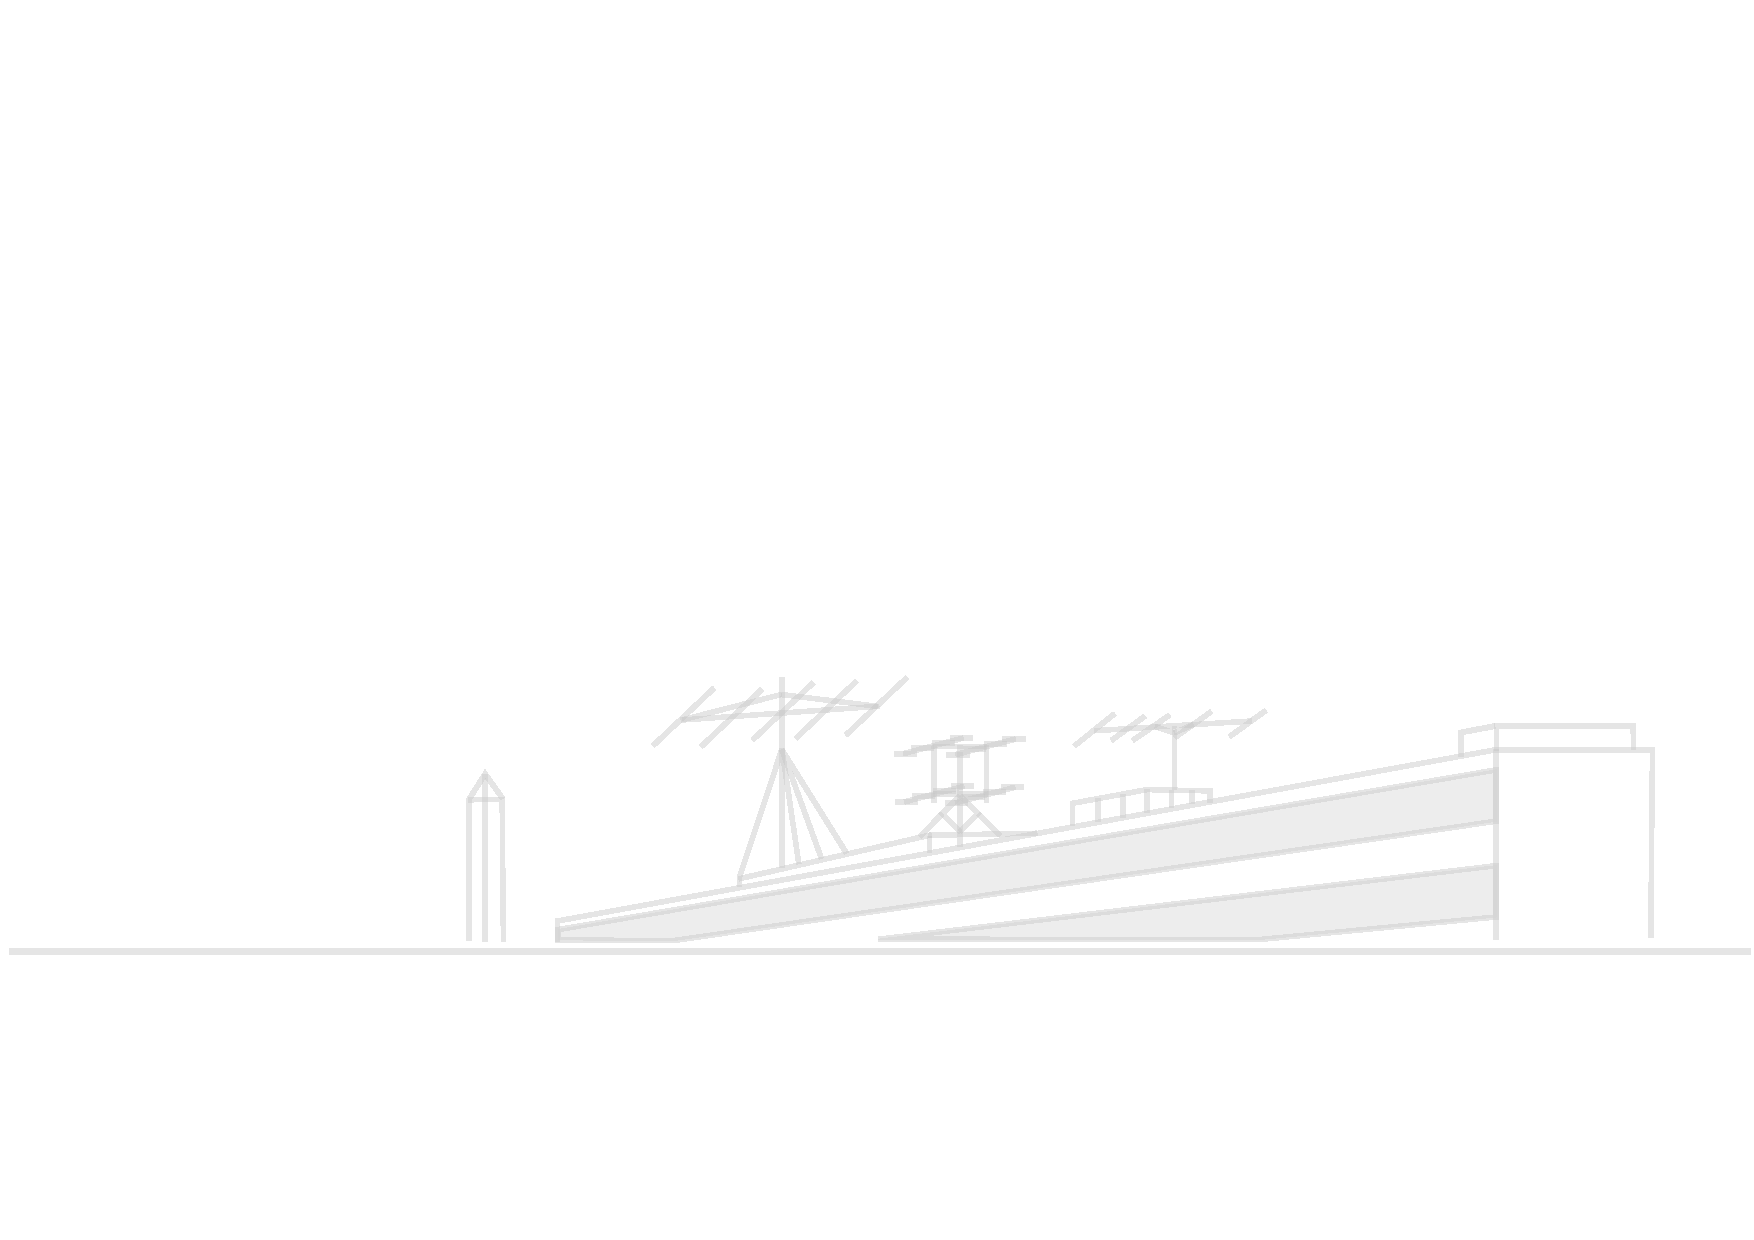
\includegraphics[width=17.8cm]{texdata/dk0tu_rooftop_background.pdf}
}

% Foliennummer einfügen
\setbeamertemplate{footline}[frame number]
%\setbeamertemplate{footline}{}

% Ändere das Zeichen vor jedem item
%\setbeamertemplate{itemize item}{\color{craneorange}$\blacktriangleright$}
%\setbeamertemplate{itemize subitem}{\color{craneorange}$\triangleright$}
%\setbeamertemplate{itemize subsubitem}{\color{craneorange}$\blacktriangleright$}

% Ändert die Blöcke 
\setbeamertemplate{blocks}[rounded][shadow=true]
% default | rounded [shadow=true|false]

%
% Eigene Kommandos
%

% Hack to get natbib and beamer working together. "The beamer user guide suggests
% that only the manual bibliography entry approach is supported"
% on some system it works out of the box, sometimes you need the hack :-(
% so check it --dl7bst
\ifdefined\newblock
    \relax
\else
    \newcommand{\newblock}{}
\fi

% \includedia command to generate png out of a dia file
% NEEDS installed dia and pdflatex option --shell-escape
\newcommand{\includedia}[1]{
    \immediate\write18{/usr/bin/dia #1.dia -e #1_diatmp.png -t png}
}

% RICHIG GROSSER FONT!
\newfont{\bigfont}{cmr10 at 144pt}
\newfont{\smallfont}{cmr10 at 8pt}

% Römische Ziffern
\makeatletter
\newcommand{\rmnum}[1]{\romannumeral #1}
\newcommand{\Rmnum}[1]{\expandafter\@slowromancap\romannumeral #1@}
\makeatother

% Schwarze Überschrift
%\setbeamercolor{frametitle}{fg=black}
%\setbeamercolor{title}{fg=black}

% Item- und Box-Farben
\definecolor{deepBlue}{HTML}{000066}
\setbeamercolor{itemize item}{fg=deepBlue}
\setbeamercolor{itemize subitem}{fg=deepBlue}
\setbeamercolor{description item}{fg=deepBlue}
\setbeamercolor{block title}{fg=deepBlue!100, bg=blue!15}
\setbeamercolor{block body}{fg=black, bg=blue!5}
\setbeamercolor{block title alerted}{fg=deepBlue, bg=red!75}
\setbeamercolor{block body alerted}{fg=black, bg=red!15}
\setbeamercolor*{block title example}{fg=blue!50, bg=blue!10}
\setbeamercolor*{block body example}{fg= blue, bg=blue!5}

%\setbeamercolor{section in head/foot}{parent=palette primary}
%\setbeamercolor{subsection in head/foot}{parent=palette secondary}
%\setbeamercolor{sidebar}{fg=darkblue,bg=yellow!90!orange}
%\setbeamercolor{title in sidebar}{fg=darkblue}
%\setbeamercolor{author in sidebar}{fg=darkblue}
%\setbeamercolor{section in sidebar}{fg=darkblue!10!black}
%\setbeamercolor{subsection in sidebar}{fg=darkblue!50!black}

% Titlepage Infos
\title{AFu-Kurs nach DJ4UF}
\author[DKØTU]{DKØTU\\ \footnotesize{Amateurfunkgruppe der TU Berlin}}
\institute[DKØTU]{\url{http://www.dk0tu.de} }

% PDF-Eigenschaften
\subject{DK0TU-Amateurfunkkurs nach DJ4UF}
\keywords{Amateurfunk Kurs HAM Radio Course CC-BY-NC-SA OpenSource TU Berlin DK0TU}

\subtitle{Technik Klasse A 13: \\
Frequenzaufbereitung \\[2em]}
\date{Stand 17.06.2016}
 \begin{document}

\begin{frame}
    \titlepage
    \vfill
    \begin{center}
        \ccbyncsaeu\\
        {\tiny This work is licensed under the \em{Creative Commons Attribution-NonCommercial-ShareAlike 3.0 License}.}\\[0.5ex]
         \tiny Amateurfunkgruppe der Technische Universität Berlin (AfuTUB), DKØTU
         %\includegraphics[scale=0.5]{img/DK0TU_Logo.pdf}
    \end{center}
\end{frame}


% FIXME Blockschaltbilder sollten in Klasse E schon irgendwo rein

\section{Überblick}

\begin{frame}
  \frametitle{Blockschaltsymbole}
  In dieser Lektion werden häufig Blockschaltsymbole verwendet. Diese stellen logisch ganze Baugruppen dar.

  \begin{center}
    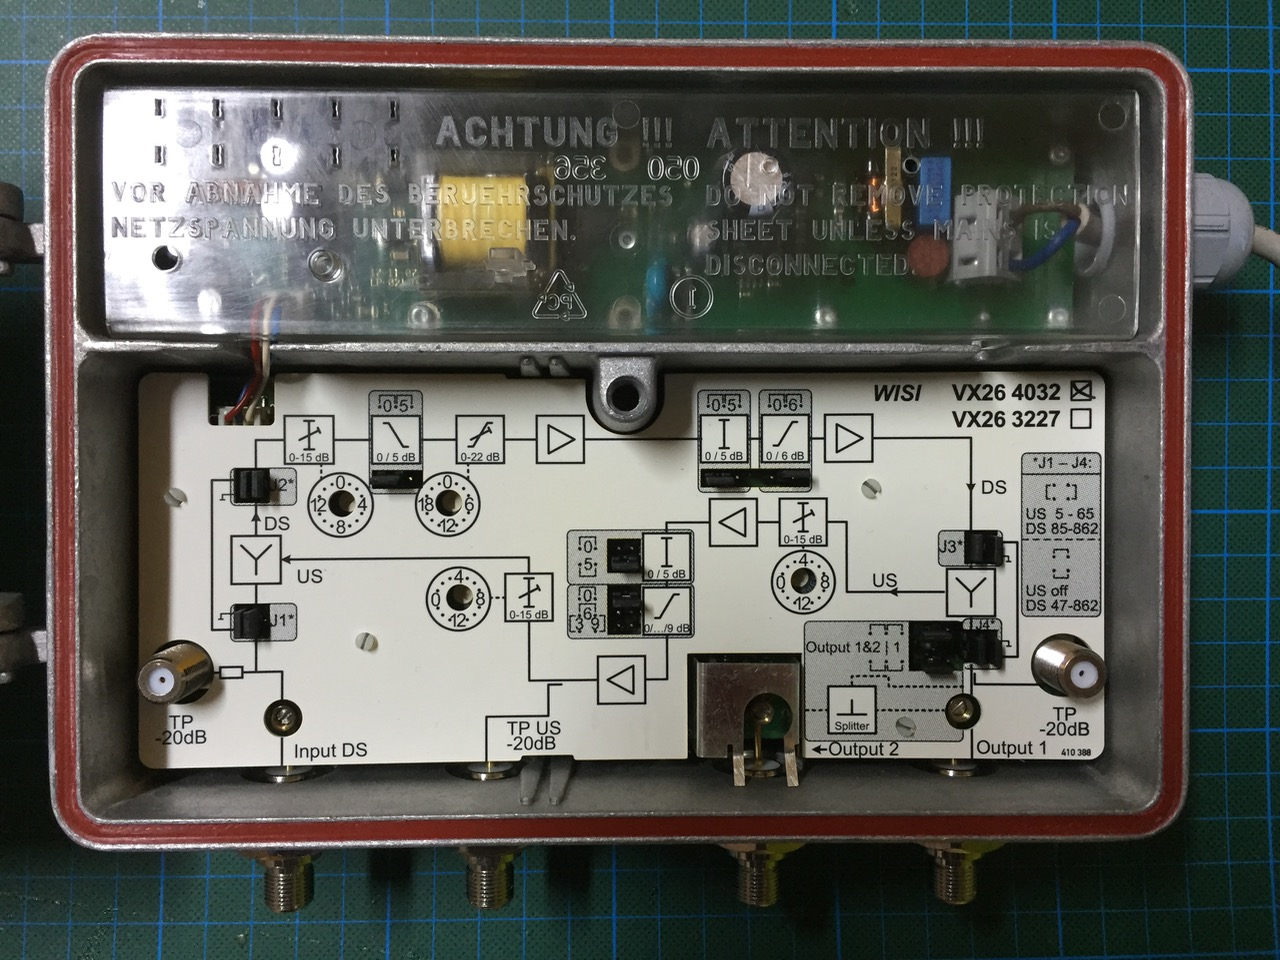
\includegraphics[width=\textwidth,height=.65\textheight,keepaspectratio]{a13/IMG_4686.jpg}\\
    {\small Hausanschlussverstärker des Kabelfernsehen mit Blockschaltbildern} {\tiny (Eigene Aufnahme DC4LW)}
  \end{center}
\end{frame}

\begin{frame}
  \frametitle{Überblick}

  Bereits bekannt aus Kapitel \emph{E15}: \\[2em]

  Signal im Basisband muss für die Übertragung auf einen HF-Träger
  ``aufgeprägt'' werden.
\end{frame}

\begin{frame}
  \frametitle{Überblick}

  Wozu Frequenzaufbereitung?\\[2em]
  Wo liegen die klassischen Kurzwellenbänder und
  was fällt dabei auf?

\end{frame}

\begin{frame}
  \frametitle{Überblick}

  ``Klassische'' Amateurfunkbänder: \\[2em]

  3,5 -- 7 -- 14 -- 21 -- 29 -- 145 -- 435 MHz (80m, 40m, 20m, 15m, 10m, 2m, 70cm)
  \only<2>{$3,5 \times2 \rightarrow 7 \times2 \rightarrow 14 \times1,5 \rightarrow 21 \times1,5 \rightarrow 29 \times5 \rightarrow 145 \times3 \rightarrow 435$ MHz}

  \vspace{3em}

  Außerdem später hinzu gekommen: \\[2em]

  1,8 -- 5 -- 10 -- 18 -- 25 -- 50 (160m, 60m, 30m, 17m, 12m, 6m)


\end{frame}

\section{Sender}

\subsection{Vervielfacher}

\begin{frame}
  \frametitle{Frequenzvervielfacher}

  \begin{columns}
    \column{.5\textwidth}
    \begin{center}
      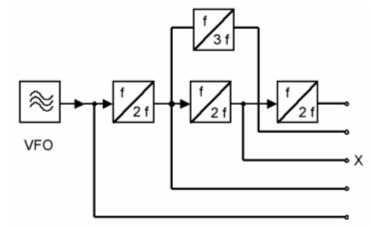
\includegraphics[width=\textwidth,height=.85\textheight,keepaspectratio]{a13/TG103a.png}
      {\tiny (TG103)}
    \end{center}
    \column{.45\textwidth}
    \begin{itemize}
      \item Oberwellen bleiben in Amateurfunkbändern
      \item Senderaufbau durch Frequenzvervielfacher
      \item aufbauend auf stabilen 3,5MHz Oszillator
    \end{itemize}
  \end{columns}
\end{frame}

\begin{frame}
  \begin{tabular}{l||p{.8\textwidth}}\hline
    \textbf{TG103} & \textbf{Das Blockschaltbild stellt einen Mehrbandsender dar. Welche Frequenz entsteht am Ausgang X, wenn der VFO auf 3,51 MHz eingestellt ist?}

    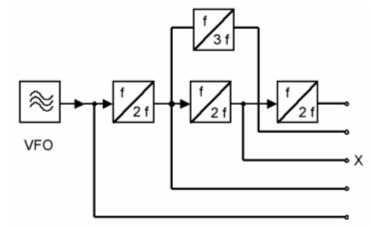
\includegraphics[width=.8\textwidth,height=.6\textheight,keepaspectratio]{a13/TG103a.png}\\ \hline \hline
    A & 3,55 MHz. \\ \hline
    B & 7,02 MHz. \\ \hline
    C & 21,06 MHz. \\ \hline
    D \only<2>\checkmark & 14,04 MHz. \\ \hline
  \end{tabular}
\end{frame}


\begin{frame}
  \frametitle{Frequenzvervielfacher}

  Bei FM darauf achten, dass sich auch der Hub vervielfacht!

  \begin{center}
    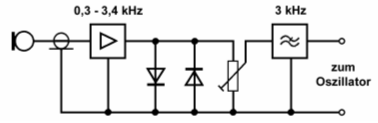
\includegraphics[width=0.8\textwidth,height=.5\textheight,keepaspectratio]{a13/TG102.png}
    {\tiny (TG102)}
  \end{center}

  Abhilfe z.B. durch Antiparallelschaltung von Dioden.\footnote{Einstellung durch
  den Widerstand}

\end{frame}

\subsection{Mischer}

\subsubsection{Einfachmischer}

\begin{frame}
  \frametitle{Einfachmischer}

  Vervielfachung ist nur bei CW und FM sinnvoll. Hub zeigt, dass Modulation ``auseinandergezogen wird'' -- bei SSB würde das Seitenband auch entsprechend vervielfacht werden und der Abstand zum Träger gerät größer.

  \begin{center}
    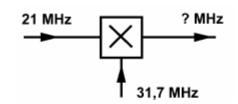
\includegraphics[width=0.5\textwidth,height=.5\textheight,keepaspectratio]{a13/TG226.png}
    {\tiny (TG226)}
  \end{center}

  Mischer sind bereits aus der Modulation bekannt. Anwendung hier:
  Up-/Downconversion.
\end{frame}

\begin{frame}
  \begin{tabular}{l||p{.8\textwidth}}\hline
    \textbf{TG226} & \textbf{Welche wesentlichen Ausgangsfrequenzen erzeugt die in der Abbildung dargestellte Stufe?}

    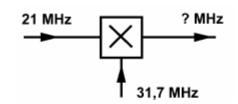
\includegraphics[width=.6\textwidth,height=.4\textheight,keepaspectratio]{a13/TG226.png} \\ \hline\hline
    A & 21,4 und 105,4 MHz \\ \hline
    B & 42 und 53,4 MHz \\ \hline
    C & 21 und 63,4 MHz \\ \hline
    D \only<2>\checkmark & 10,7 und 52,7 MHz \\ \hline
  \end{tabular}
\end{frame}

\begin{frame}
  \frametitle{Einfachmischer}

  \begin{center}
    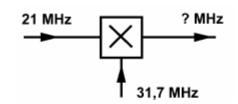
\includegraphics[width=0.5\textwidth,height=.5\textheight,keepaspectratio]{a13/TG226.png}
    {\tiny (TG226)}
  \end{center}

  \begin{itemize}
    \item das unerwünschte Mischprodukt muss gut gefiltert werden
    \item eine Mischfrequenz wird von einem Quarzoszillator \textbf{CO} (crystal oscillator) hinzugefügt
    \item die andere Mischfrequenz wird von einem \textbf{VFO} (variable frequency oscillator) hinzugefügt
    \item damit wird die Ausgangsfrequenz variabel
  \end{itemize}
\end{frame}

\begin{frame}
  \begin{exampleblock}{Mischung}
    CO = $9 MHz$\\
    VFO = $5,0\cdots5,5MHz$
    \vspace{2em}
    \pause
    \begin{align*}
      f_{H 5,0} &= 9 MHz + 5,0 MHz = 14,0 MHz & f_{H 5,5} &= 9 MHz + 5,5 MHz = 14,5 MHz \\
      f_{L 5,0} &= 9 MHz - 5,0 MHz = 4,0 MHz  & f_{L 5,5} &= 9 MHz - 5,5 MHz = 3,5 MHz \\
    \end{align*}
  \end{exampleblock}
  \pause
  Welche Bänder sind das?
\end{frame}


\subsubsection{Balance-Mischer}

\begin{frame}
  \frametitle{Balance-Mischer}

  SSB-Aufbereitung mit einem 9-MHz-Quarzfilter (balancierter Ringmischer)

  \begin{center}
    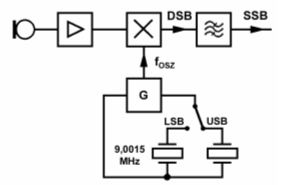
\includegraphics[width=0.5\textwidth,height=.5\textheight,keepaspectratio]{a13/TG106.png}
    {\tiny (TG106)}
  \end{center}

  {\small CO LSB: $9,0015MHz$; CO USB: $8,9985MHz$}\\[.5em]

  Ein fester Bandpassfilter bei $9MHz$ mit $\pm1,2kHz$ Bandbreite lässt nur eines der beiden Seitenbänder durch.

\end{frame}

\begin{frame}
  \frametitle{Balance-Mischer}

  Der gesamte Sendepfad würde so aussehen:

  \begin{center}
    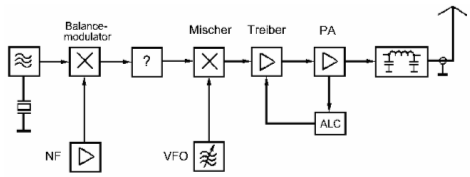
\includegraphics[width=0.8\textwidth,height=.5\textheight,keepaspectratio]{a13/TG101.png}
    {\tiny (TG101)}
  \end{center}

  Was wird nach der SSB-Mischstufe benötigt?
  \vspace{2em}
  \pause

  Ein Quarzfilter als Seitenbandsperre.

\end{frame}

\subsection{Mehr"-fach"-mischer"-prinzip}
\begin{frame}
  \frametitle{Mehrfachmischerprinzip}
  \begin{itemize}
    \item es gibt einen nicht umschaltbaren VFO
    \item Mischung mit der erzeugten SSB-Filterfrequenz
    \item erzeugt eine Zwischenfrequenz (ZF)
    \item die ZF wird durch Mischung zur Endfrequenz für die Antenne gebracht
  \end{itemize}
\end{frame}

\subsection{VCO-PLL}

\begin{frame}
  \frametitle{Phasenregelung}

  Phasenregelschleifen dienen zum Angleichen zweier Phasen.

  \bigskip

  Hier: \textbf{VCO-PLL} (voltage controlled oscillator phase locked loop)

\end{frame}

\begin{frame}
  \frametitle{VCO-PLL}

  \begin{center}
    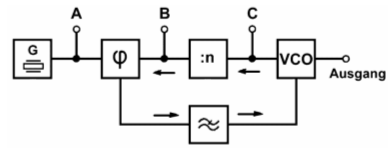
\includegraphics[width=0.8\textwidth,height=.4\textheight,keepaspectratio]{a13/TD701.png}
    {\tiny (TD701)}
  \end{center}

  \only<1>{
  \begin{itemize}
    \item VCO (voltage-controlled oscillator) ist das Herzstück
    \item Quarzgenerator erzeugt Referenzfrequenz
    \item Teilerfunktion ``:n'' steuert die Ausgangsfrequenz (heutzutage oft von Mikroprozessor)
    \item Phasenkomparator $\varphi$
    \item stabiler Zustand: Die Frequenzen an A und B sind gleich
    \item der Tiefpass erzeugt eine Gleichspannung vom Mittelwert des Pulses an C
  \end{itemize}
  }
  \only<2>{
  \begin{itemize}
    \item bei Phasenverschiebung der Frequenzen ergibt sich im Komparator ein Signal mit kürzeren oder längeren Pausen zwischen den Impulsen
    \item dadurch verschiebt sich die Spannung über den Tiefpass
    \item der VCO erhält eine andere Spannung und regelt nach
  \end{itemize}
  }
  \only<3>{
  \begin{itemize}
    \item die VCO-PLL ``lockt'' auf ein Vielfaches der Quarzoszillatorfrequenz ein
    \item der Teiler bestimmt die größe der Ausgangsfrequenz
  \end{itemize}
  }
\end{frame}

\begin{frame}
  \begin{tabular}{l||p{.8\textwidth}}\hline
    \textbf{TD706} & \textbf{Die Frequenz am Punkt A beträgt 12,5 kHz. Es sollen Ausgangsfrequenzen im Bereich von 12,000 MHz bis 14,000 MHz erzeugt werden. Welchen Bereich muss der Teilerfaktor umfassen?}

    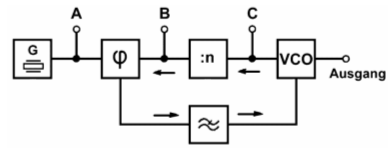
\includegraphics[width=.7\textwidth,height=.5\textheight,keepaspectratio]{a13/TD701.png} \\ \hline\hline
    A & 300 bis 857 \\ \hline
    B & 300 bis 1120 \\ \hline
    C & 960 bis 857 \\ \hline
    D \only<2>\checkmark & 960 bis 1120 \\ \hline
  \end{tabular}
  \pause
  \vspace{.5em}
  $n_1 = \frac{12000kHz}{12,5kHz} = 960$ --- $n_2 = \frac{14000kHz}{12,5kHz} = 1120$
\end{frame}


\subsubsection{Mehrfach-Mischer}

\begin{frame}
  \frametitle{Mehrfach-Mischer}

  % TODO Muendl. oder Folien warum Mehrfachmischung

  \begin{columns}[c]
    \column[c]{.6\textwidth}
    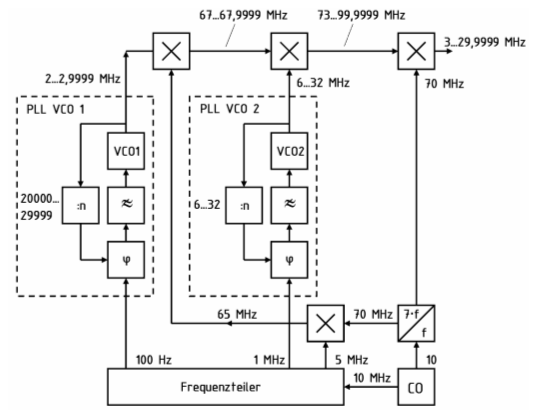
\includegraphics[width=\textwidth,height=.85\textheight,keepaspectratio]{a13/TG110.png}
    {\tiny (TG110)}
    \column{.35\textwidth}
    \begin{itemize}
      \item Nur ein CO
      \item zwei PLL-Schleifen
      \item Aufmischung zwischen $3\cdots30MHz$ möglich
    \end{itemize}
  \end{columns}
\end{frame}

\begin{frame}
  \begin{tabular}{l||p{.8\textwidth}}\hline
    \textbf{TG110} & \textbf{Im folgenden Blockschaltbild ist die Frequenzaufbereitung für einen Amateurfunk-Transceiver dargestellt. Welche Frequenz erzeugt der Sender, wenn VCO1 auf 2,651\,MHz eingestellt und VCO2 auf 6\,MHz eingerastet ist?}

    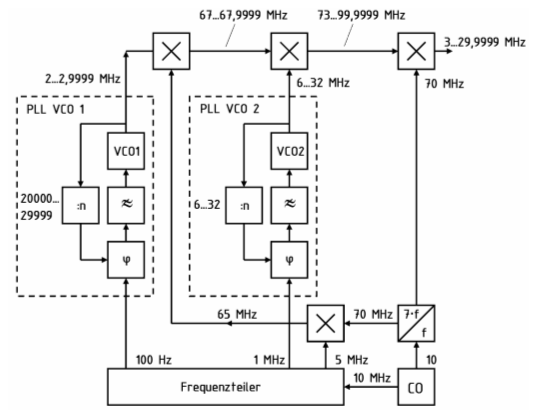
\includegraphics[width=.55\textwidth,height=.55\textheight,keepaspectratio]{a13/TG110.png} \\ \hline\hline
    A & 6,651 MHz \\ \hline
    B \only<2>\checkmark & 3,651 MHz \\ \hline
    C & 8,651 MHz \\ \hline
    D & 14,351 MHz \\ \hline
  \end{tabular}
\end{frame}


\section{Empfänger}

\begin{frame}
  \frametitle{Empfängerprinzipien}

  Doppelsuper: Niedrige zweite Zwischenfrequenz (ZF) gute Trennschärfe. \\[2em]

  Bei heutigen TRX: Die 1.\,ZF liegt höher als das Doppelte der maximalen
  Empfangsfrequenz. Nach der Filterung im Roofing-Filter (1.\,ZF) wird auf die
  2.\,ZF im Bereich um 9 bis 10\,MHz heruntergemischt. \\[2em]

  Erste ZF-Filterbandbreite mind. so groß wie höchste benötigte Bandbreite.
\end{frame}

\begin{frame}
  \frametitle{Spiegelfrequenz}
  \begin{block}{Unerwünschte Frequenz beim Runtermischen auf die Zwischenfrequenz}
    $f_S = f_E + 2 \cdot f_{ZF} \text{ für } f_{OSZ} > f_E$ \\
    $f_S = f_E - 2 \cdot f_{ZF} \text{ für } f_{OSZ} < f_E$
  \end{block}
  Unterdrückung möglich durch
  \begin{itemize}
    \item geringe Bandbreite (Bandpassfilter am Eingang)
    \item Phasenverfahren (Mischung mit der phasengedrehten Spiegelfrequenz)
    \item Spiegelfrequenz weit außerhalb des Empfangsbereichs erzeugen (oder sogar unter 0Hz)
  \end{itemize}
\end{frame}

\subsection{Doppelsuper}

\begin{frame}
  \begin{tabular}{l||p{.8\textwidth}}\hline
    \textbf{TF201} & \textbf{In dieser Schaltung können bei einer Empfangsfrequenz von 145,6\,MHz und einer Oszillatorfrequenz von 134,9\,MHz Spiegelstörungen auftreten. Berechnen Sie diese Spiegelfrequenz.}

    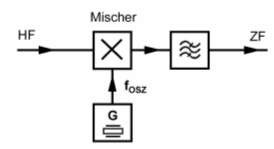
\includegraphics[width=0.5\textwidth,height=.5\textheight,keepaspectratio]{a13/TF201.png}\\ \hline\hline
    A & 156,3 MHz \\ \hline
    B & 134,5 MHz \\ \hline
    C \only<2>\checkmark & 124,2 MHz \\ \hline
    D & 280,5 MHz \\ \hline
  \end{tabular}
  \pause
  \vspace{1em}
  $f_{ZF} = f_{HF} - f_{osz} \rightarrow f_{SP} = f_{osz} - f_{ZF} \text{ bei } f_{osz} < f_{HF}$
\end{frame}

\begin{frame}
  \frametitle{Doppelsuper}

  \begin{center}
    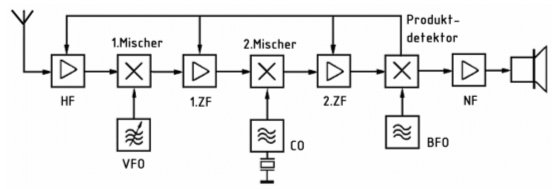
\includegraphics[width=0.8\textwidth,height=.5\textheight,keepaspectratio]{a13/TF205b.png}
    {\tiny (TF205b)}
  \end{center}

  \begin{itemize}
    \item 1. ZF relativ hoch (oft um 10,7\,MHz) $\rightarrow$ gute Spiegelfrequenzunterdrückung
    \item 2. ZF niedrig (oft um 460\,kHz) $\rightarrow$ hohe Trennschärfe
  \end{itemize}
\end{frame}

\begin{frame}
  \begin{tabular}{l||p{.8\textwidth}}\hline
    \textbf{TF205} & \textbf{Ein Doppelsuper hat eine erste ZF von 10,7\,MHz und eine zweite ZF von 460\,kHz. Die Empfangsfrequenz soll 28\,MHz sein. Welche Frequenz ist für den VFO und für den CO erforderlich, wenn die Oszillatoren oberhalb des Nutzsignals schwingen sollen?}

    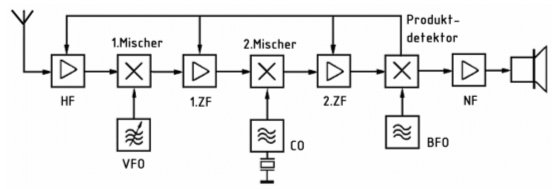
\includegraphics[width=.6\textwidth,height=.5\textheight,keepaspectratio]{a13/TF205b.png} \\ \hline\hline

    A & Der VFO muss bei 38,70\,MHz und der CO bei 12,24\,MHz schwingen. \\ \hline
    B & Der VFO muss bei 10,24\,MHz und der CO bei 17,30\,MHz schwingen. \\ \hline
    C \only<2>\checkmark & Der VFO muss bei 38,70\,MHz und der CO bei 11,16\,MHz schwingen. \\ \hline
    D & Der VFO muss bei 28,46\,MHz und der CO bei 11,16\,MHz schwingen.\\ \hline
  \end{tabular}
  \pause
  \vspace{.5em}
  \begin{scriptsize}
    \begin{align*}
      \text{VFO: } 28MHz + 10,7MHz &= 38,7MHz\\
      \text{CO: } 10,7MHz + 460kHz &= 11,16MHz
    \end{align*}
  \end{scriptsize}
\end{frame}

\begin{frame}
  \frametitle{Doppelsuper}

  \begin{center}
    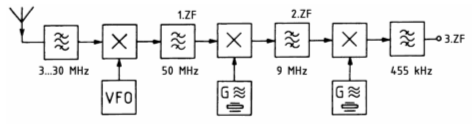
\includegraphics[width=0.8\textwidth,height=.5\textheight,keepaspectratio]{a13/TF209b.png}
    {\tiny (TF209b)}
  \end{center}

  Vorteil von Kurzwellen-Empfängern mit sehr hoher ZF (z.B. 50 MHz):
  Spiegelfrequenz liegt sehr weit außerhalb des Empfangsbereichs.

\end{frame}


\subsection{Direkt"-über"-lagerungs"-empfänger}

\begin{frame}
  \frametitle{Direktüberlagerungsempfänger}

  Auch Produktdetektor genannt. \\[2em]

  Prinzip wie der Einfachmischer beim TX. Eine Mischstufe mit VFO in nächster
  Nähe zur Empfangsfrequenz.

\end{frame}

\subsection{PLL}

\begin{frame}
  \frametitle{PLL}

  \begin{center}
    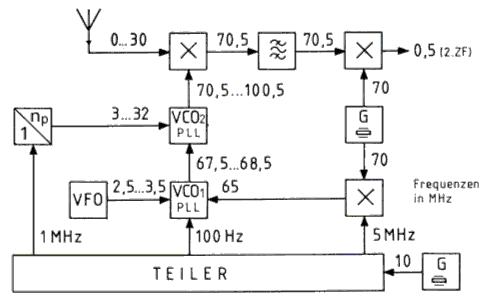
\includegraphics[width=0.8\textwidth,height=.7\textheight,keepaspectratio]{a13/TF213.png}
    {\tiny (TF213)}
  \end{center}

  Prinzip wie beim Sender
\end{frame}

\begin{frame}
  \begin{tabular}{l||p{.8\textwidth}}\hline
    \textbf{TF213} & \textbf{Dies ist das Blockschaltbild eines modernen Empfängers mit PLL-Frequenzaufbereitung. Es soll eine Frequenz von 15,0\,MHz emfangen werden. Welche Frequenzen liefern $VCO_1$ und $VCO_2$, wenn der programmierbare Frequenzvervielfacher $n_p$ dabei 18\,MHz liefert?}

    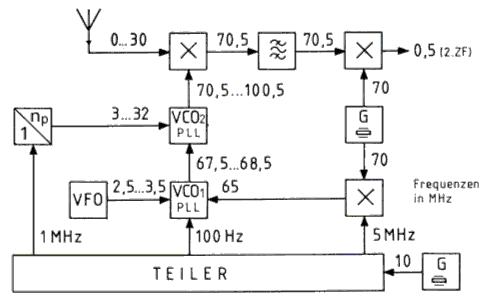
\includegraphics[width=0.48\textwidth,height=.48\textheight,keepaspectratio]{a13/TF213.png}\\ \hline\hline
    A & $VCO_1$: 67,5\,MHz, $VCO_2$: 87,5\,MHz \\ \hline
    B & $VCO_1$: 68,5\,MHz, $VCO_2$: 88,5\,MHz \\ \hline
    C & $VCO_1$: 88,5\,MHz, $VCO_2$: 67,5\,MHz \\ \hline
    D \only<2>\checkmark & $VCO_1$: 67,5\,MHz, $VCO_2$: 85,5\,MHz \\ \hline
  \end{tabular}
\end{frame}


\subsection{Converter}

\begin{frame}
  \frametitle{Converter}

  \begin{center}
    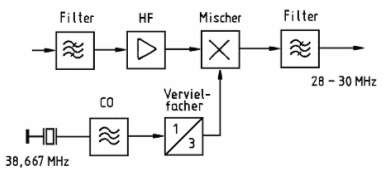
\includegraphics[width=0.8\textwidth,height=.7\textheight,keepaspectratio]{a13/TF204.png}
    {\tiny (TF204)}
  \end{center}

  2-m-Konverter für einen KW-Empfänger

\end{frame}

\subsection{Transverter}

\begin{frame}
  \frametitle{Transverter (Transceiver-Konverter)}

  \begin{center}
    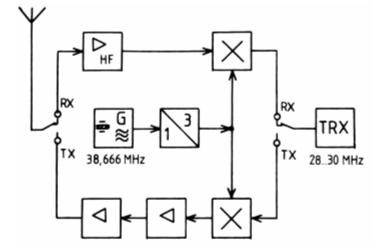
\includegraphics[width=0.8\textwidth,height=.7\textheight,keepaspectratio]{a13/TF209.png}
    {\tiny (TF209)}
  \end{center}

  Transverter für das 2-m-Band

\end{frame}

\renewcommand{\refname}{Referenzen}

\hypertarget{refs}{}
\textcolor{white}{} \\ %\vspace{} geht nicht
\Large Referenzen/Links
\footnotesize

\begin{thebibliography}{}
  \bibitem{darc}  DARC Online-Lehrgang Lektion A13:
    \url{https://www.darc.de/der-club/referate/ajw/lehrgang-ta/a13/}
  \bibitem{bna}   Fragenkatalog Bundesnetzagentur Technik Klasse A:\\
    \url{https://www.bundesnetzagentur.de/SharedDocs/Downloads/DE/Sachgebiete/Telekommunikation/Unternehmen_Institutionen/Frequenzen/Amateurfunk/Fragenkatalog/TechnikFragenkatalogKlasseAf252rId9014pdf.pdf?__blob=publicationFile&v=3}
\end{thebibliography}

% Hier könnte noch eine Kontaktfolie stehen

\end{document}

